\begin{figure}[H]
    \centering
    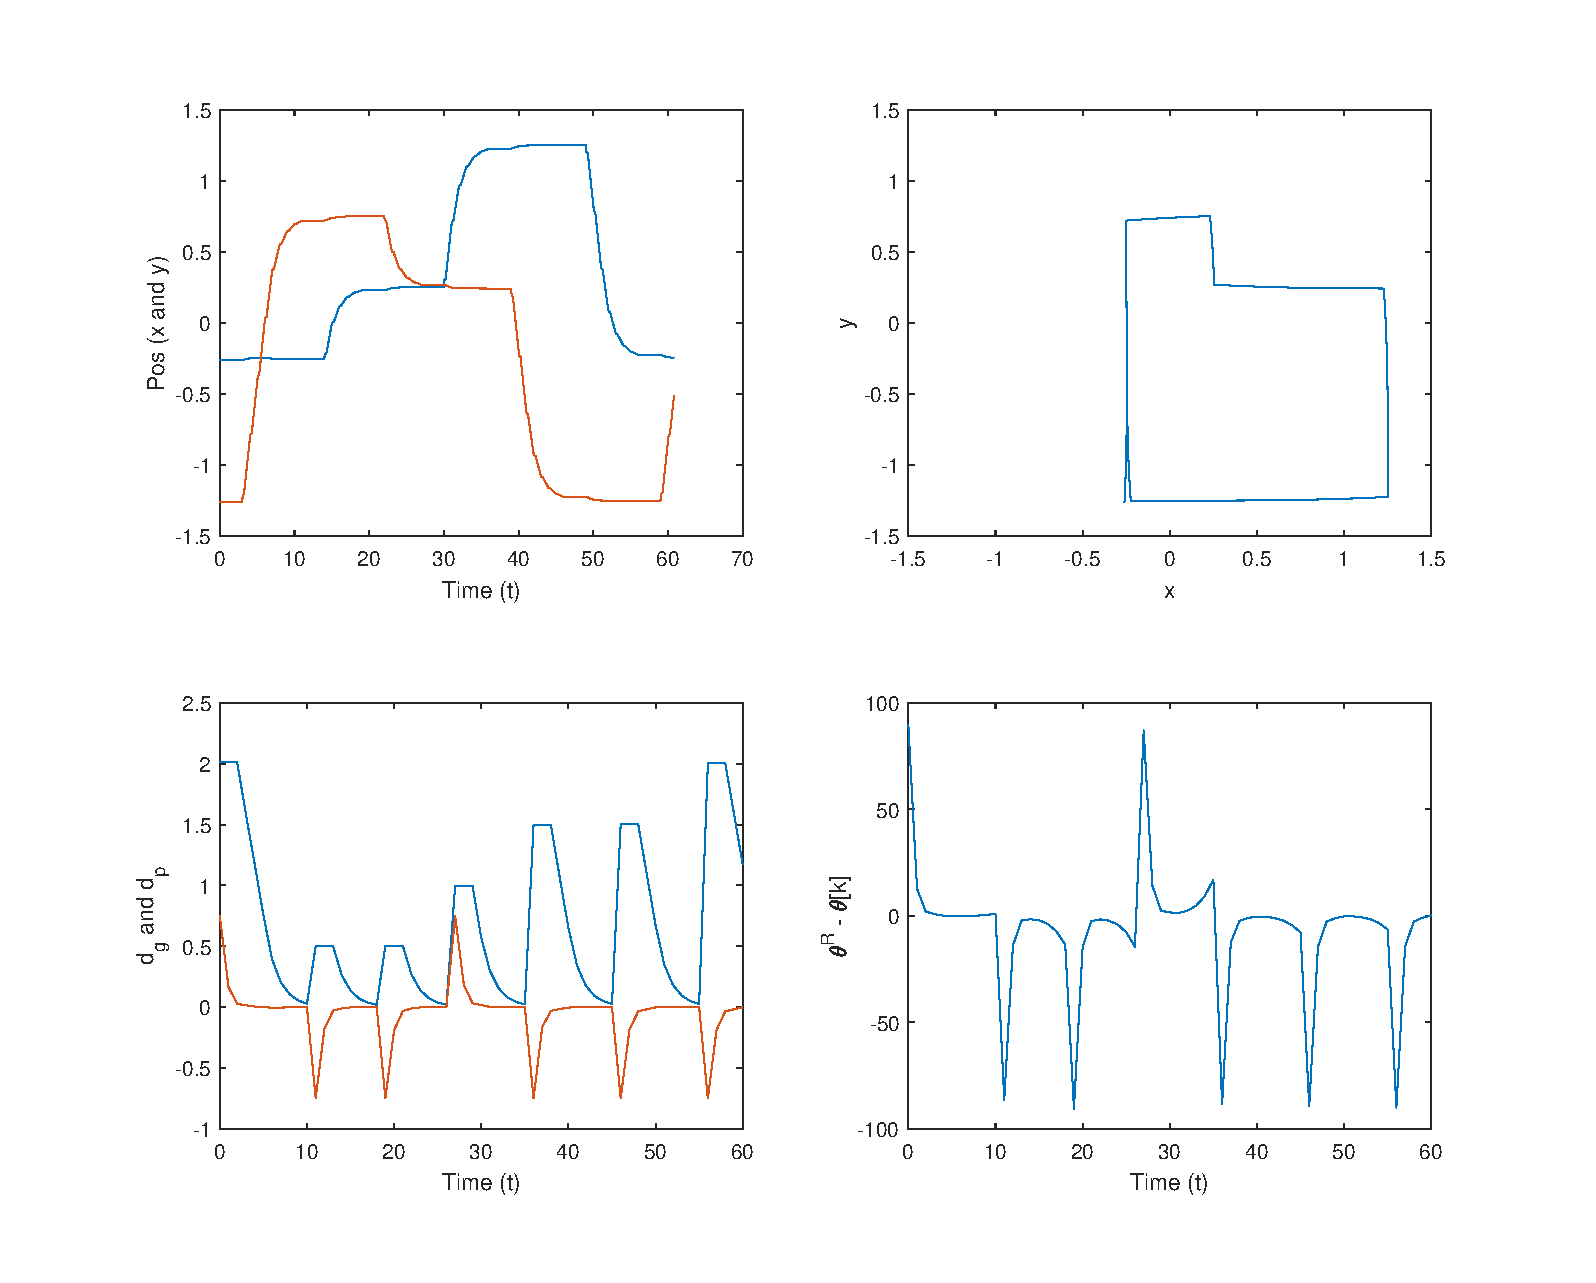
\includegraphics[width=\textwidth]{figs/perf-fullrun.eps}
    \caption{Simulation of a full run with the hybrid controller going from $(0, 0)$ to $(2, 2)$ with $K_\omega = \frac{180}{R\pi}$, and $p = 0.75.$ The directional controller has $K_\psi = \frac{L}{R}$ and the got to goal controller uses $K_\psi = \frac{180}{\pi} \frac{L}{Rp}$} \label{fig:perf-full}
\end{figure}

\begin{figure}[H]
    \centering
    \includegraphics[width=\textwidth]{figs/states-full.eps}
    \caption{The sequence of discrete states of the hybrid controller for a full run. } \label{fig:states-full}
\end{figure}

As can be seen in figure \ref{fig:perf-full}, the robot performed reasonably well. There are some concerns that the behavior is a bit uncontrolled, which might have caused it to occasionally cross into a forbidden state. A plot displaying the robots full radius from the path combined by a grid showing the states would have been interesting.

